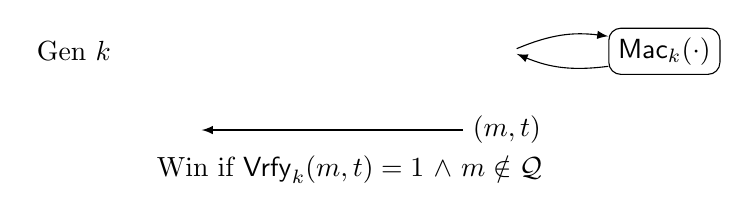
\begin{tikzpicture}
\node (A) at (0,0) {\Homer};
\node (B) [right of = A, node distance = 4cm] {\Left\Burns};
\node (enc) [draw, rounded corners=1ex, right of=B, node distance = 2cm] {$\mathsf{Mac}_k(\cdot)$};
\draw[-latex] (B) to [bend left=15,-latex,above] (enc);
\draw[-latex] (enc) to [bend left=15,-latex,below] (B);
\node (k) [left of=A, node distance = 1.5cm] {Gen $k$};
\node (1a) [below of=A, node distance=1cm] {};
\node (1b) [below of=B, node distance=1cm] {$(m,t)$};
\draw[-latex] (1b) -- (1a) node [midway,above] {};
%\node (2a) [below of=1a, node distance=0.5cm] {Gen $b$};
%\node (2b) [below of=1b, node distance=0.5cm] {};
%\draw[-latex] (2b) -- (2a) node [midway,above] {};
%\node (3a) [below of=2a, node distance=0.5cm] {};
%\node (3b) [below of=2b, node distance=0.5cm] {};
%\node (4a) [below of=2a, node distance=0.5cm] {$\mathsf{Enc}_k(m_b)$};
%\node (4b) [below of=2b, node distance=0.5cm] {};
%\draw[-latex] (4a) -- (4b) node [midway,above] {};
%\node (5a) [below of=4a, node distance=0.5cm] {};
%\node (5b) [below of=4b, node distance=0.5cm] {$b'$};
%\draw[-latex] (5b) -- (5a) node [midway,above] {};
\node (6a) [below of=1a, node distance=0.5cm] {};
\node (6b) [below of=1b, node distance=0.5cm] {};
\node (result) [right of = 6a, node distance = 2cm] {Win if $\mathsf{Vrfy}_k(m,t)=1$ $\land$ $m \notin \mathcal{Q}$};
\end{tikzpicture}
